%
% Bachelor Thesis
% Sven Hodapp
%


% -----------
% 1. Präambel
% -----------


% Allgemeine Einstellungen
% ------------------------
\documentclass[
	pdftex,%              PDFTex verwenden da wir ausschliesslich ein PDF erzeugen.
	a4paper,%             Wir verwenden A4 Papier.
	oneside,%             Einseitiger Druck.
	12pt,%                Grosse Schrift, besser geeignet für A4.
	halfparskip,%         Halbe Zeile Abstand zwischen Absätzen.
	%chapterprefix,%       Kapitel mit 'Kapitel' anschreiben.
	headsepline,%         Linie nach Kopfzeile.
	footsepline,%         Linie vor Fusszeile.
	bibtotocnumbered,%    Literaturverzeichnis im Inhaltsverzeichnis nummeriert einfügen.
	idxtotoc%             Index ins Inhaltsverzeichnis einfügen.
]{report}

\usepackage[utf8]{inputenc}
\usepackage[german]{babel}   % deutsche Silbentrennung
\selectlanguage{german}   % damit Table Of Contents Inhaltsverzeichnis genannt wird

\usepackage{geometry}   % Seitenränder einstellbar
\usepackage{textcomp}   % Sonderzeichen, wie Eurosymbol



% Bilder, Farben, farbige Tabellen
% --------------------------------
\usepackage{graphicx, color, colortbl}
\usepackage{longtable}
\usepackage{lscape}
\usepackage{array}       % Erweiterte Tabelleneigenschaften.
%\usepackage{floatflt}   % Bild kann von Text umflossen werden.



% Palatino Schrift
% ----------------
%\usepackage[T1]{fontenc}
%\usepackage[osf]{mathpazo}   % osf aktiviert Mediävalziffern/Minuskelziffern



% Syntax-Highlighting
% -------------------
% Src: http://tihlde.org/~eivindw/latex-listings-for-scala/
\definecolor{dkgreen}{rgb}{0,0.6,0}
\definecolor{gray}{rgb}{0.5,0.5,0.5}
\definecolor{mauve}{rgb}{0.58,0,0.82}

\usepackage{listings}

% "define" Scala
\lstdefinelanguage{Scala}{
  morekeywords={abstract,case,catch,class,def,%
    do,else,extends,false,final,finally,%
    for,if,implicit,import,match,mixin,%
    new,null,object,override,package,%
    private,protected,requires,return,sealed,%
    super,this,throw,trait,true,try,%
    type,val,var,while,with,yield},
  otherkeywords={=>,<-,<\%,<:,>:,\#,@},
  sensitive=true,
  morecomment=[l]{//},
  morecomment=[n]{/*}{*/},
  morestring=[b]",
  morestring=[b]',
  morestring=[b]"""
}

\lstset{
  frame=tb,
  language=Scala,
  aboveskip=3mm,
  belowskip=3mm,
  showstringspaces=false,
  columns=flexible,
  basicstyle={\small\ttfamily},
  numbers=left,
  numberstyle=\tiny\color{gray},
  keywordstyle=\color{blue},
  commentstyle=\color{dkgreen},
  stringstyle=\color{mauve},
  frame=single,
  breaklines=true,
  breakatwhitespace=true,
  tabsize=2,
  extendedchars=\true,
  inputencoding=utf8,
  escapeinside={\%*}{*)}  % http://tex.stackexchange.com/questions/24528/
}


% Sonstige Pakete
% ---------------
%\usepackage{anysize}   % Seitenränder verändern
%\usepackage{setspace}   % 1.5em Zeilenabstand \begin{onehalfspacing}
\usepackage{bibgerm}   % Anzeigestil des Literaturverzeichnis (gerabbrv)
\usepackage{paralist}  % Individualisierte Aufzählungen


% Definition von globalen Konstanten
% ----------------------------------
\newcommand{\thema}{
	Vergleich von interner und externer DSL-Technologie zur Entwicklung
	eines Textsatzsystems zur automatischen Dokumentengenerierung.}
\newcommand{\schlagworte}{DSL, Dokumentengenerierung}
\newcommand{\zusammenfassung}{
	Im Zuge dieser Bachelor-Thesis wird ein zeitgemäßer Ansatz für ein
Texsatzsystem entwickelt und auf die Probe gestellt, als Vorbild dient \TeX.

	Kerntechnologien sind HTML5, CSS3 und Javascript zur Gestaltung und
Darstellung eines Dokuments, das dabei entstehende Framework ermöglicht
semi-automatische Dokumentengenerierung. Zur Generierung der eigentlichen
Dokumenteninhalte werden zwei verschiedene DSL Ansätze Verglichen, zum einen
eine interne Scala-DSL, zum anderen eine externe DSL mit dem Xtext-Framework.

	Vorteile gegenüber \TeX sollen sein: Flexibles Dokument-Templating und
interaktive Dokument-Elemente, ermöglicht durch die ubiquitäre
HTML-Technologie. Ein moderneres und mächtigeres Sprachkonzept als es
\LaTeX bietet, mit allen Finessen einer kompletten und verbreiteten
Programmiersprache.}
\newcommand{\ausgabedatum}{16.10.2012}
\newcommand{\abgabedatum}{16.01.2013}
\newcommand{\autor}{Sven Hodapp}
\newcommand{\autorStrasse}{Hohentwielstraße 2}
\newcommand{\autorPLZ}{78247 }
\newcommand{\autorOrt}{Hilzingen}
\newcommand{\autorGeburtsort}{Singen/Hohentwiel}
\newcommand{\autorGeburtsdatum}{16.09.1987 }
\newcommand{\prueferA}{Prof. Dr. Marko Boger}
\newcommand{\prueferB}{Dr. Marc Zimmermann}
\newcommand{\firma}{Fraunhofer-Institut für Algorithmen und
Wissenschaftliches Rechnen SCAI}
\newcommand{\studiengang}{Software-Engineering}




% PDF Eigenschaften
% -----------------
\usepackage
[
	colorlinks=false,
	bookmarks = true,
	pdftitle={\thema},
	pdfauthor={\autor},
	pdfsubject={Bachelor Thesis},
	pdfkeywords={\schlagworte},
	urlcolor=blue,
	pdfstartview=FitH
]{hyperref}





% --------------------
% 2. Dokumenten Anfang
% --------------------

\begin{document}

\pagenumbering{roman}

% Deckblatt
% ---------

\begin{titlepage}

\vspace*{-3.5cm}

\begin{flushleft}
\hspace*{-1cm} 
\includegraphics[width=15.7cm]{titlepages/htwg-logo}
\end{flushleft}

\vspace{2.5cm}

\begin{center}
	\huge{
		\textbf{\thema} \\[4cm]
	}
%\normalsize{\textbf{(Working Draft)} \\}
	\Large{
		\textbf{\autor}} \\[4cm]
	\large{
		\textbf{Konstanz, \abgabedatum} \\[1cm]
	}
	\Huge{
		\textbf{{\sf BACHELORARBEIT}}
	}
\end{center}

\end{titlepage}

\setcounter{page}{2}
\thispagestyle{empty}
{
\setlength{\parskip}{0.5cm}
        \begin{center}
        \textbf{\huge BACHELORARBEIT}

        \textbf{zur Erlangung des akademischen Grades}

        \textbf{\Large Bachelor of Science (B. Sc.)}

        \textbf{an der}

        \textsf{\huge Hochschule Konstanz}\\
        {\small Technik, Wirtschaft und Gestaltung}

        \textsf{\Large Fakult"at Informatik} \\
        Studiengang \studiengang
        \end{center}
}
\begin{center}

\vspace*{2cm}

\begin{tabular}{p{3cm}p{10cm}}
Thema: & \textbf{\large \thema} \\[15ex]
Bachelorkandidat: & \autor, \autorStrasse, \autorPLZ  \autorOrt \\[15ex]
1. Pr"ufer: & \prueferA \\
2. Pr"ufer: & \prueferB \\[25ex]
Ausgabedatum: & \ausgabedatum \\
Abgabedatum: & \abgabedatum \\
\end{tabular}
\end{center}


\begin{center}
{\Large \textbf{Zusammenfassung (Abstract)}}
\end{center}

\bigskip

\begin{center}
	\begin{tabular}{p{2.8cm}p{10cm}}
		Thema: & \thema \\
		 & \\
		Bachelorkandidat: & \autor \\
		 & \\
		Firma: & \firma \\
		 & \\
		Betreuer: & \prueferA  \\[.5ex]
		 &  \prueferB \\
		 & \\
		Abgabedatum: & \abgabedatum \\
		 & \\
		Schlagworte: & \schlagworte \\
		 & \\
	\end{tabular}
\end{center}

\bigskip

\noindent
\zusammenfassung
\chapter*{Ehrenw"ortliche Erkl"arung}
\addcontentsline{toc}{chapter}{Ehrenw"ortliche Erkl"arung}

Hiermit erkl"are ich
\textit{\autor, geboren am \autorGeburtsdatum in \autorGeburtsort}, dass ich\\

\begin{tabular}{lp{12cm}}
(1) & meine Bachelorarbeit mit dem Titel \\[1em]
& \textbf{\thema} \\[1em]
& bei der \firma\ unter Anleitung von \prueferA\ selbst"andig und ohne fremde Hilfe angefertigt und keine anderen als die angef"uhrten Hilfen benutzt habe;\\[1em]
(2) & die "Ubernahme w"ortlicher Zitate, von Tabellen, Zeichnungen, Bildern und
Programmen aus der Literatur oder anderen Quellen (Internet) sowie die Verwendung
der Gedanken anderer Autoren an den entsprechenden Stellen innerhalb der Arbeit
gekennzeichnet habe.\\
\end{tabular}

\vspace*{1cm}

\noindent
Ich bin mir bewusst, dass eine falsche Erkl"arung rechtliche Folgen haben wird.\\

\vspace*{3cm}

\noindent
Konstanz, \abgabedatum \hfill \begin{tabular}{c} \\ \\ \rule{5cm}{1pt} \\ (Unterschrift)\end{tabular}




% Inhaltsverzeichnis anzeigen
% ---------------------------
\tableofcontents
\newpage

\pagenumbering{arabic}

% ---------
% 3. Inhalt
% ---------

\chapter{Einleitung}

Die Idee entstammt der Zeit als ich mein Praxissemester beim Fraunhofer ISE
gemacht habe, da die Tools zur automatischen Dokumentengenerierung, genauer
den Jahresbericht, alle weniger geeignet erschienen. Die gewünschten
Fähigkeiten müssen über mehrere Tools zusammenlaufen, welche nicht immer
ideal zusammenarbeiten; z.B. LaTeX plus Microsoft Word. Ab da an tüftelte
ich daran, wie diesem Umstand Besserung gelingen kann.

Wie schon erwähnt handelt es sich um ein Tool, welches automatische
Dokumentengenerierung ermöglichen soll. Für diese oder ähnliche Aufgaben
gibt es bereits zahlreiche andere Werkzeuge wie z.B.:

\begin{itemize}
  \item LaTeX,
  \item Word, OpenOffice,
  \item Google Docs,
  \item ...
\end{itemize}

Jedes dieser Werkzeuge hat seine individuellen Vor- und Nachteile.
Aber diese Bachelor-Thesis will einen anderen Ansatz ausprobieren, und
seine Machbarkeit, Praxistauglichkeit und Weiterentwicklungsmöglichkeiten
festzustellen bzw. zu überprüfen.

\section{Idee}

Wie wäre es, wenn als Dokument-Endprodukt eine HTML/CSS/JS-Webseite
herauskommt? Wenn dieses Endprodukt zudem vom Webbrowser aus passend auf
eine DIN-A4-Seite gedruckt oder als PDF gespeichert werden kann?

Wie wäre es, wenn als Dokumenten-\-Generator-\-Sprache eine \emph{vollwertige}
Programmiersprache zum Einsatz käme? Wenn diese Sprache zudem an die
Domänen\-gege\-ben\-heit die durch den Willen ein Dokument zu verfassen geprägt ist?

Was kann man alles damit anstellen?

\begin{itemize}
  \item Vermischung von statischen und automatisch generierten
        Doku\-menten-\-Be\-stand\-teilen,
  \item Datenaufbereitung quasi zur Laufzeit der Doku\-menten-\-Er\-stell\-ung,
  \item Strukturierungsmöglichkeiten durch den Quellcode, in Pakete, Klassen
        → Objekt-Orientierung,
  \item Webtechnologie ermöglicht dynamische Inhalte,
  \item Webtechnologie ist reaktiv (z.B. auf den Benutzer, Inhalte nachladen),
  \item Gute Kolloberationsmöglichkeiten, Verwaltungsmöglichkeiten,
        da Quellcode
  \item Verknüpfung verschiedener Technologien (Datenbanken, Dateisystem,
        Interpozesskommunikation, etc.),
  \item Sehr flexible Gestaltung des Dokuments, da Webtechnologie möglich,
  \item Webtechnologie ermöglicht Rückkanal, z.B. kollaborierende Benutzer
        können Kommentare schreiben, oder mehr. (Richtung Google Docs.),
  \item Viele Erweiterungsmöglichkeiten, geg. durch Programmiersprache und
        Webtechnologie,
  \item Webtechnologie hat eine sichere Zukunft und ist standardisiert.
\end{itemize}

Es muss also ein kleines JavaScript-Framework entwickelt werden, welches die
Aufgabe der Darstellung des Dokuments übernimmt. Die Zielachitektur.

Zudem braucht es noch ein Programm bzw. Programmiersprache, welches diese
Zielarchitektur füttern kann. Dieses Programm soll Aufgaben wie z.B.
Kapitel-Nummerierung automatisch abwickeln. Weiterhin muss es auch ein
wohlgeformte Schnittstelle zum Benutzer liefern. Diese Kriterien führen
dazu, dass die Entwicklung einer Domänen-Spezifischen Programmiersprache,
kurz DSL, sehr sinnvoll ist.

\section{Eine Wendung}

Als ich soweit an der Thematik getüftelt hatte und die Machbarkeit als
Bachelor-Thesis erkannte trug ich den Vorschlag am ISE vor, jedoch sind
diese kein Informatik Institut und sahen sich nicht in der Lage die Arbeit
zu betreuen, wenngleich sie die Idee sehr nützlich fanden. So wurde mir
nahe gelegt, dass ich bei einem anderen Fraunhofer Institut anklopfen könne.

Ich habe das Fraunhofer SCAI angeschrieben, und Dr. Marc Zimmermann fand
die Idee spannend und auch passend für deren Themengebiet. Sie bereiten u.a.
Patente auf, indem sie eine Patent-PDF-Datei mit Hilfe ihres Java-Framework
zerlegen und die so erhaltenen Daten ggf. mit zusätzlichen Informationen
anreichern. Die Idee von mir hat ihnen sehr zugesagt, da sie noch eine
Möglichkeit suchten, die die aufbereiteten Patente mit Webtechnologie
darzustellen kann bzw. auszuliefern.

\section{Zum Dokument}

In diesem Dokument versuche ich nach Möglichkeit \emph{vollständig}
deutsche Sprache anzuwenden, also nur dort wo es unumgänglich ist
Anglizismen zu verwenden. Das gilt auch gerade für Fachsprache, sofern es
passende deutsche Übersetzungen gibt.

\chapter{Anwendungsfall: Problembeschreibung}

In diesem Kapitel soll eine umfassende Beschreibung des Problems erfolgen,
aus welcher sich wiederum die Aufgabenstellung ergibt. Diese dann im
späteren Verlauf umgesetzt wird.

Den Anfang macht die Zielachitektur, welche primär aus Webtechnologien
besteht und somit zur Darstellung des Dokumentes dient. Siehe
Abschnitt \ref{sec-zielarchitektur}.

Die Zielarchitektur soll von einem Benutzer ohne großen Aufwand
generierbar sein und dabei die Möglichkeit haben, bestimmte
Aufgaben automatisch zu erledigen, wie z.B. das Zusammenstellen
eines Inhaltsverzeichnisses. Siehe Abschnitt \ref{sec-dsl}.

Damit aus der Schnittstelle die dem Benutzer gegebenen ist die Zielarchitektur
generiert werden kann, muss es eine geeignete Brücke bzw. Verbindung
geben, welche in Abschnitt \ref{sec-verbindung} näher beschrieben wird.

\section{Allgemeiner Aufbau von Dokumenten}

Vor allem akademische Dokumente wie z.B. Bücher, Patente oder Bachelorarbeiten
haben alle im Groben einen ähnlichen Aufbau. Daher ist es sinnvoll erst einmal
allgemeine Ableitung über die Struktur solcher Dokumente zu machen, so dass
später daraus eine Architektur für nachfolgende Implementierungen entstehen kann.

Die wichtigsten Unterteilungen,
  wie auf Abbildung \ref{fig-areal_pages_entities} dargestellt,
werden hier grob definiert als

\begin{itemize}
  \item Dokumenten\emph{areal}.
        Beispielsweise gliedert sich diese Bachelorarbeit in die
        Areale Titelseiten, Inhaltsverzeichnis, Hauptdokument, Anhang und
        Literaturverzeichnis auf.
  \item Seiten.
        Jedes Dokument kann eventuell verschiedenartige Seiten haben, aber zumindest
        eine Standardseite, wie z.B. vertikales DIN A4, muss vorhanden sein.
        Aber auch innerhalb des Dokuments kann es verschiedenartige Seiten
        geben, wie z.B. horizontale Seiten für extra bereite Tabellen oder
        Titelblätter mit speziellem Layout.
  \item Entitäten.
        Das sind die einzelnen Einheiten wie Überschriften, Texte, Tabellen
        oder Bilder woraus sich schlussendlich das Dokument zusammensetzt.
\end{itemize}

\begin{figure}[h!]
  \centering
    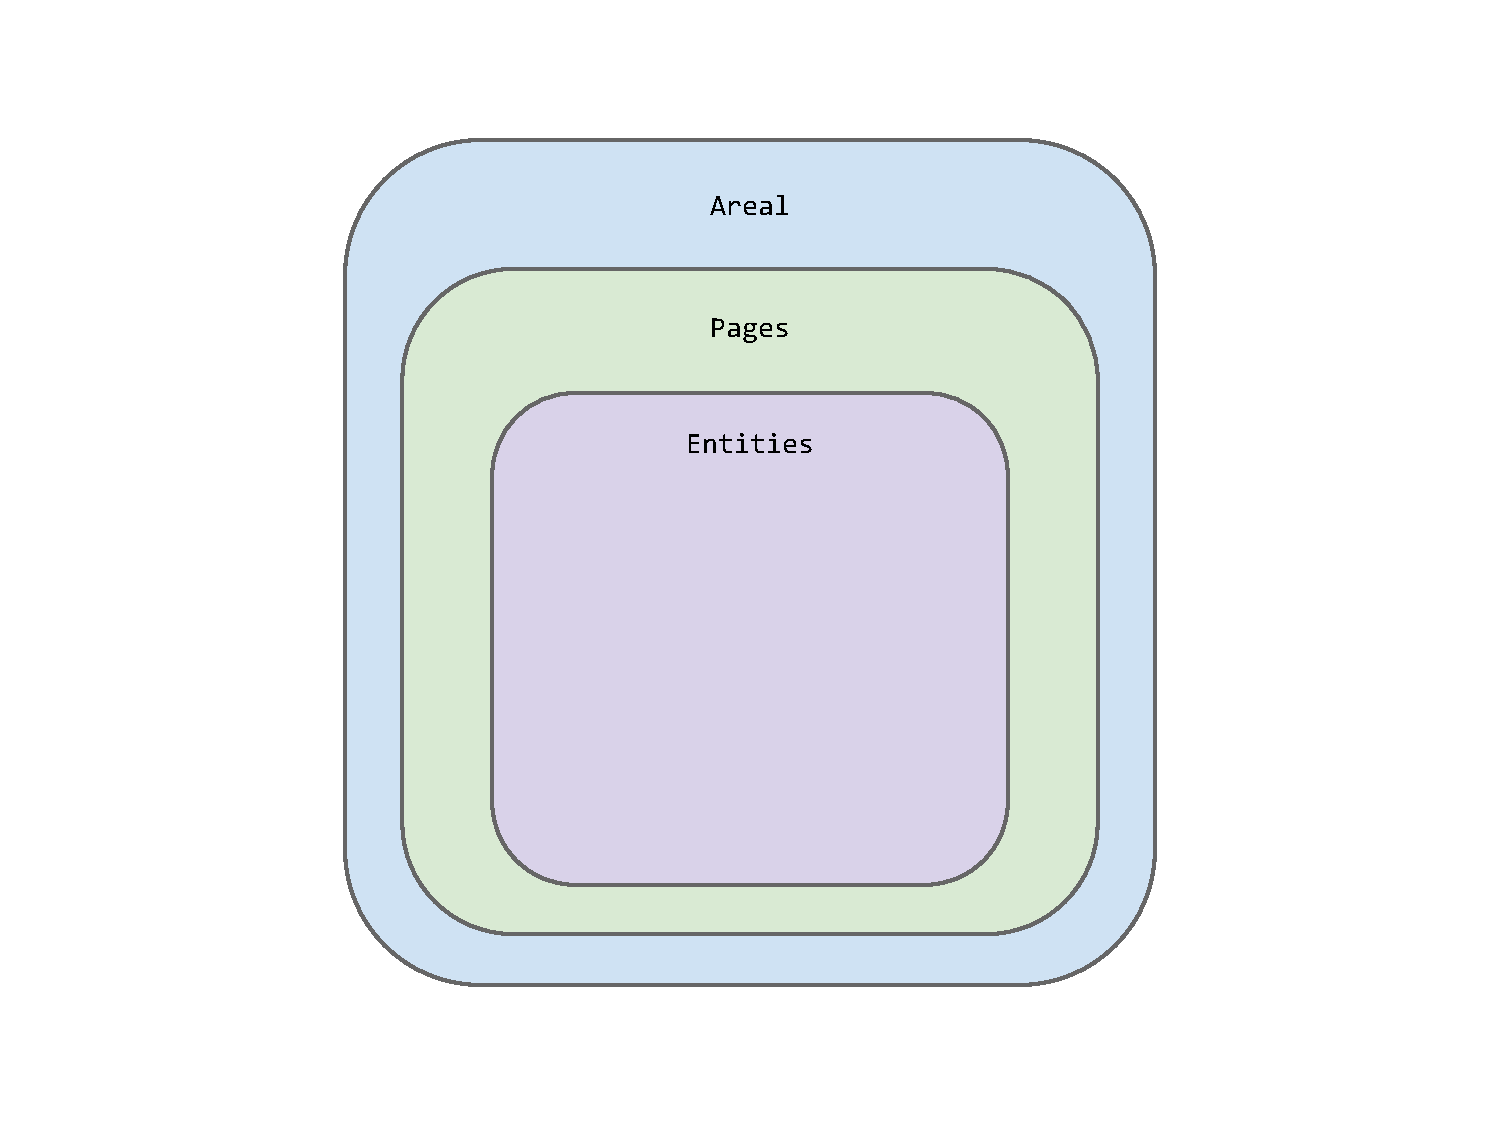
\includegraphics[width=0.9\textwidth]{figures/areal_pages_entities.pdf}
  \caption{Ein Dokument kann hierarchisch grob in Areal, Seiten und Entitäten gegliedert werden.}\label{fig-areal_pages_entities}
\end{figure}

\section{Zielarchitektur}\label{sec-zielarchitektur}

Die primäre Aufgabe der Zielarchitektur ist es ein Dokument in
einem Webbrowser darzustellen. Das Dokument ist aber keine gewöhnliche
Webseite, sondern orientiert sich hautsächlich an akademischen
Dokumenten wie z.B. Fachbüchern. Bücher bestehen aus einzelnen Seiten,
welche in Webseiten in ihrer Ursprünglichen Form nicht vorgesehen sind.
Lange Dokumente werden mit Webtechnologie für gewöhnlich stufenlos
dargestellt, also alles auf einer einzelnen „Seite.“
Daher ist die Hauptaufgabe der Zielarchitektur eine \emph{Abstraktion
über Seiten} für Webtechnologie zu schaffen.

Die eigentliche Problematik ist hierbei, dass der Webbrowser fließenden
Text nicht selbst auf definierte Seiten umbrechen kann. Für den Browser
gibt es nur eine Seite, die quasi einem langen Textschlauch entspricht,
wenngleich er durch HTML strukturiert und
CSS-Eigenschaften gestaltet werden kann.

Damit verbunden ist die Problematik der
\emph{Zuordnung der einzelnen Dokumenten-Entitäten zu den Seiten},
dabei kann es dazu kommen dass eine Entität zwischen zwei Seiten
\emph{überlappt} und diese sollte, wenn möglich passend aufgeteilt werden.

Dadurch dass die Zielarchitektur sich um die Erstellung der Seiten und
die Zuteilung der Entitäten kümmern muss, ist es vollkommen natürlich,
dass sich diese auch der \emph{Durchnummerierung der Seiten} annehmen muss.
Davon hängt auch direkt die Funktion, die einzelnen Punkte des
Inhaltsverzeichnisses mit der entsprechenden Seitennummer zu versehen, ab.

Zudem sollte es möglich sein, dass es \emph{verschiedene Arten von Seiten}
gibt, z.B. Deckblatt, normale vertikale Seite und horizontale Seiten für
große Tabellen oder Abbildungen. Oder auch dass verschiedene Papierformate
wie DIN-A4 oder US-Letter zur Auswahl stehen.

Die Einführung von \emph{Dokumenten-Arealen} als eine weitere hilfreiche
Abstraktion die zur Gliederung eines -- insbesondere
akademischen -- Dokuments dient, ist mit Sicherheit wünschenswert.
Damit soll es möglich sein, Dinge wie beispielsweise
Deckblatt, Inhaltsverzeichnis, eigentliches Dokument
und Literaturverzeichnis etc. von einander zu separieren, um für eine
flexiblere Konfiguration zu bieten. Beispielsweise um Areale in der Anordnung zu
verändern, oder Dinge wie Nummerierungen zu modifizieren, es wird z.B.
gerne der Anfang eines Dokuments mit römischen Ziffern durchnummeriert
und das eigentliche Dokument jedoch mit arabischen Ziffern.

% Seitennummerierung
% Inhaltsverzeichnis, Seite zuordnen
% Dokumentenareale
% Vorteile die sich durch die HTML-Nutzung ergeben? Welches Kapitel?

\paragraph{Aufgaben} auf einen Blick zusammengefasst:

\begin{itemize}
  \item Abstraktion für Seiten,
  \item Zuordnung der Entitäten auf Seiten,
  \item Behandlung überlappender Entitäten,
  \item Ermöglichung verschiedener Seiten-Arten,
  \item Durchnummerierung der Seiten,
  \item Seitenzugehörigkeit von Entitäten bestimmbar,
  \item Dokumenten-Areale zur Strukturierung.
\end{itemize}


\section{Domain-Specific Language}\label{sec-dsl}

Die \emph{domain-specific language}, kurz \emph{DSL}, stellt die
textuelle Schnittstelle zwischen Benutzer und der Zielplatform dar.
Eine DSL ist eine leichtgewichtige Programmiersprache, die für den
Einsatz ihres Spezialgebietes, ihrer Domäne bzw. ihres Aktionsraumes,
zugeschnitten ist.

Dabei unterscheidet man grob zwischen \emph{internen}, \emph{externen}
und \emph{nicht-textuellen} DSLs.\cite{dsls} Da in diesem Projekt allerdings
nur eine textuelle DSL zum Einsatz kommen soll, konzentrieren wir uns
auf die internen DSLs bzw. externen DSLs.

\paragraph{Definition interne DSL}
\begin{quote}
Eine interne DSL wird als Bibliothek auf Basis
einer bereits existierenden Wirtssprache implementiert. Das interne DSL-Skript
ist eine dünne Fassade über die Abstraktionen der unterliegenden Wirtssprache.
\end{quote} (von \cite{dsls} Kapitel 1.5.1, Seite 18.)

\paragraph{Definition externe DSL}
\begin{quote}
Eine externe DSL wird von Grund auf entwickelt und hat eine separate
Infrastruktur für die lexikalische Analyse, Interpretation, Kompilierung
und Code Generierung. Eine externe DSL zu entwickeln ist gleichzusetzen mit
der Implementierung einer neuen Sprache von Grund auf, welche ihre eigene
Syntax und Semantik hat.
In den meisten Fällen findet man externe DSLs vor, welche nicht alle
Komplexitäten einer vollwertigen Sprache benötigt.
\end{quote} (von \cite{dsls} Kapitel 1.5.2, Seite 18f.)

\paragraph{Ausgewählt und gegenübergestellt werden}

\begin{itemize}
  \item die Scala-Programmiersprache für interne DSLs,
  \item das Xtext-Framework für externe DSLs.
\end{itemize}

Warum genau diese zwei Vertreter sich besonders eigenen und ausgewählt wurden,
wird in Kapitel \ref{sec-warumAusgewaehlt} beschrieben.

\subsection{\TeX, eine DSL für Dokumente}

\TeX~ ist eine weit verbreitete Programmiersprache die speziell für die
Aufgaben eines Textsatzsystem erschaffen wurde. Daher kann man
\TeX~ auch als eine \emph{externe DSL} ansehen.
In diesem Abschnitt wird etwas auf
\TeX~ eingegangen, da insbesondere diese Programmiersprache als Inspiration
bzw. Vorbild dient.


\subsubsection{Herkunft und Grundlagen}

Der Name hat seinen Ursprung aus dem griechischen $\tau\epsilon\chi$,
welches auch die Wurzel für das englische Wort \emph{technology} ist.
$\tau\epsilon\chi$ bedeutet also Technologie, aber auch Kunst.
(\cite{tex-a}, Kapitel 1, Seite 1)

\TeX~ ist ein Dokumenten-Compiler, welcher dazu gedacht ist hochqualitativen
Textsatz zu erstellen, mit einem starken Fokus auf
Mathematik. \TeX82 ist in der Programmiersprache Pascal-H definiert
bzw. in WEB. (\cite{tex-b}, §1, Seite 1)

Die prototypische Entwicklung begann im Sommer 1977, Version 0 wurde
im September 1982 fertig gestellt, seit dem wurde TeX eingefroren
und seither wird nur noch an der Stabilität und Zuverlässigkeit
gearbeitet. (\cite{tex-b}, §2, Seite 2)

Es gibt etwa 300 \TeX~Kontrollsequenzen, sog. „Primitive“ welche das
Low-Level TeX bilden. Diese Primitiven sind atomisch und werden nicht weiter
in kleinere Funktionen zerlegt.
Zudem kommen noch etwa 600 weitere, aus Primitiven zusammengesetzte,
Kontrollsequenzen „plain \TeX“ dazu,
die zusammen mit den Primitiven das Standard-\TeX~bilden.
(\cite{tex-a}, Kapitel 3, Seite 9--11)

\TeX~ hat eine \emph{REPL}\footnote{REPL steht für read–eval–print loop,
eine interaktive Programmierumgebung. Scala besitzt auch eine REPL.
Dieser kann unter UNIX mit dem Befehl \lstinline|tex| aufgerufen werden.}
in welcher interaktive Programmiersitzungen abgehalten werden können,
wie z.B.:

\paragraph{Primitiv}

\begin{verbatim}
**\show\input
> \input=\input.
\end{verbatim}

\paragraph{Zusammengesetzte Kontrollsequenz, ein Makro}

\begin{verbatim}
**\show\TeX
> \TeX=macro:
->T\kern -.1667em\lower .5ex\hbox {E}\kern -.125emX.
\end{verbatim}

Viele Ligaturen\footnote{Ligaturen wie z.B. \lstinline|ff| zu ff}
werden von TeX als solche erkannt und direkt also solche
im resultierenden Dokument umgesetzt. Zudem können mit einer gewöhnlichen
Tastatur auch ungewöhnliche Zeichen gesetzt werden, so kann z.B. mit der
\lstinline|\ss| \TeX-Sequenz ein ß gesetzt werden, was dem Dokument
schöne Typographie bzw. Zeichen anderer Sprachen, mit lateinischen
Zeichen, erlaubt. (\cite{tex-a}, Kapitel 9, Seite 51--52)

Jedes einzelne Zeichen ist eine Box welche, aus Höhe, Breite, Tiefe und
einer Basisline besteht, diese Boxen können
zu größeren Einheiten „verklebt“ werden, so dass daraus schlussendlich
auch komplizierte Seiten-Layouts zusammengestellt werden können.
(\cite{tex-a}, Kapitel 11, Seite 63)

\begin{figure}[h!]
  \centering
    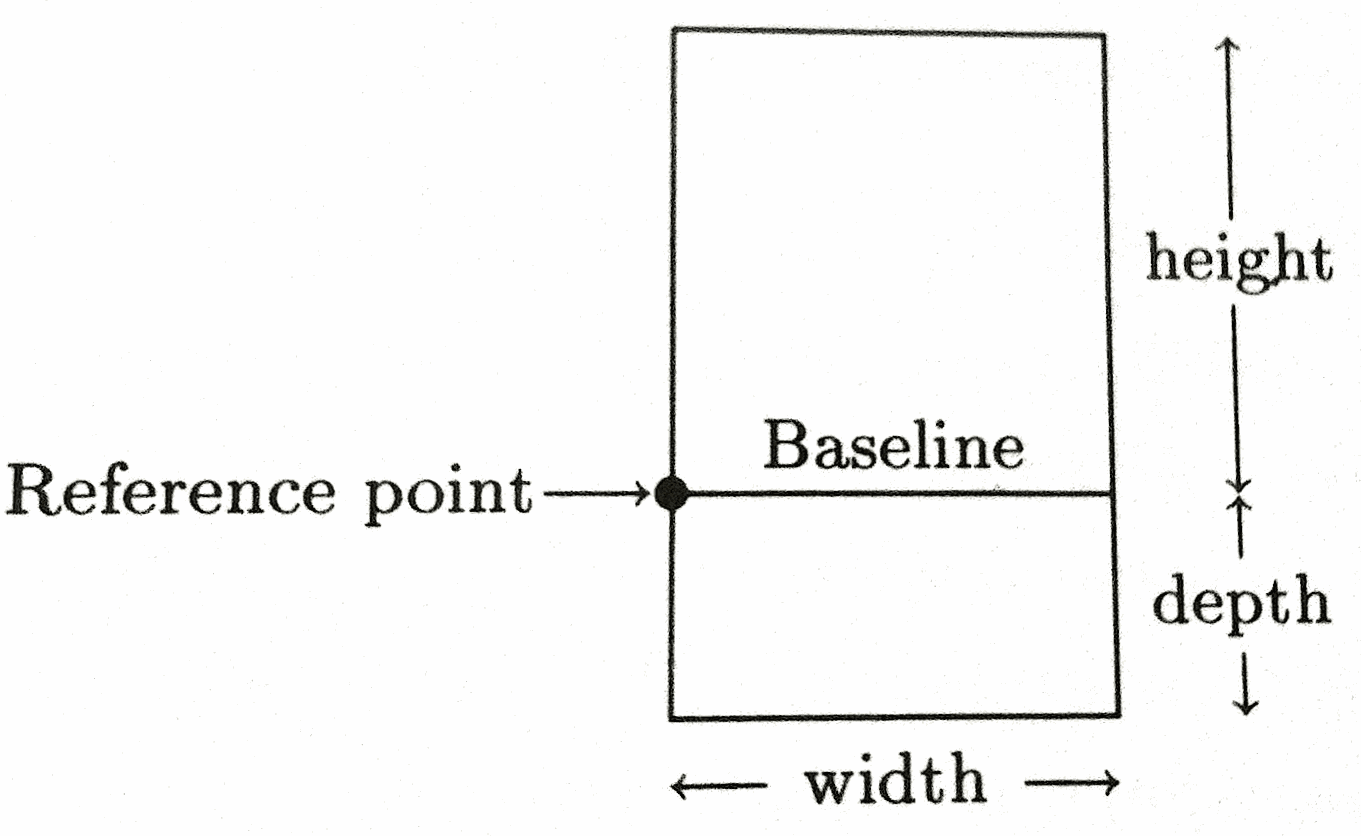
\includegraphics[width=0.5\textwidth]{figures/tex_box.png}
  \caption{\TeX~ Box für jedes einzelnes Zeichen.
           (\cite{tex-a}, Kapitel 11, Seite 63)}\label{fig-tex_box}
\end{figure}

\TeX~ kann einen Abschnitt in einzelne Zeilen herunterbrechen, so dass
der Benutzer sich nicht um diese Aufgabe kümmern muss. Es wird der beste
Weg gesucht, für den jeweiligen Abschnitt das „minimale Übel“ zu finden.
(\cite{tex-a}, Kapitel 14, Seite 91)
Die Methode die in TeX verwendet wird, geht auf Michael F. Plass
und Donald E. Knuth zurück. (\cite{tex-b}, §813, Seite 343)
Zudem ist ein Silbentrennungsalgorithmus enthalten, der auf
Frank M. Liang zurückgeht. (\cite{tex-b}, §919, Seite 386)

Das Dokument in einzelne Seiten zu unterteilen kann \TeX~ automatisch
vornehmen. Machmal ist es allerdings geschickter, wenn der Dokumentenersteller
mit etwas Handarbeit den Seitenumbruch selbst einstellt, um ein ideales
Ergebnis zu erzielen. (\cite{tex-a}, Kapitel 15, Seite 109)

\subsubsection{Fähigkeiten als Programmiersprache}

Mit den geschweiften Klammern \{ und \} sind die Gruppierungssymbole, so
dass Änderungen innerhalb einer Gruppe nicht auch Dinge außerhalb
verändern. (\cite{tex-a}, Kapitel 5, Seite 19)
Das Verhalten ist also gewohnt wie es in Programmiersprachen wie C,
Java oder Scala vorkommt.

Makros bzw. Definitionen ermöglichen es Abkürzungen für z.B. häufig
verwendete Kontrollsequenzen anzulegen, so dass insbesondere
der Quellcode übersichtlicher wird bzw. der Dokumentenersteller sich
Schreibarbeit sparen kann.

\begin{verbatim}
\def\xvec{(x_1,\ldodts,x_n)} --> \xvec
\end{verbatim}

TeX expandiert dann automatisch das Makro für den Benutzer.
So ist es sinnvoll wenn TeX-Benutzer ihre eigene kleine Bibliothek mit
Makros zusammenstellen, so dass sie diese in verschiedenen Dokumenten
wiederverwenden können. (\cite{tex-a}, Kapitel 20, Seite 199)
\LaTeX~ ist \emph{u.a.} eine sehr bekannte und beliebte
Bibliothekszusammenstellung\footnote{\url{http://www.latex-project.org}}.

\begin{verbatim}
\input macros  % Importiert aus macros.tex
\end{verbatim}

Parametrisierte Makros sind auch möglich, was TeX eine mächtige
Makroprogrammierfähigkeit verschafft:

\begin{verbatim}
\def\cs #1. #2\par{...}
\end{verbatim}

Wobei in diesem Beispiel nach Aufruf von \lstinline|\cs| Parameter
\lstinline|#1| so lange gilt,
bis \lstinline|". "| auftritt und Parameter \lstinline|#2|
bis \lstinline|'\par'| auftritt. (\cite{tex-a}, Kapitel 20, Seite 202)

Die Makros können auch rekursiv aufgebaut werden, so dass damit auch möglich ist
Schleifen (tail recursive) zu bilden.
(\cite{tex-a}, Kapitel 20, Seite 219)
TeX selbst bietet auch ein \lstinline|\loop...\repeat| Kommando an,
mit dessen Hilfe Schleifen gebildet werden können.
(\cite{tex-a}, Kapitel 20, Seite 217)


\paragraph{Einer Kontrollsequenz eine Bedeutung zuweisen:}

\begin{itemize}
  \item \lstinline|\font\cs=<font name>|
        (\lstinline|\cs| wird ein font identifier),
  \item \lstinline|\chardef\cs=<number>|
        (\lstinline|\cs| wird ein character code),
  \item \lstinline|\countdef\cs=<number>|
        (\lstinline|\cs| wird ein \lstinline|\count| register,
        was quasi einer int Variablen entspricht),
  \item \lstinline|\def\cs...{...}|
        (\lstinline|\cs| wird ein Macro),
  \item \lstinline|\let\cs=<token>|
        (\lstinline|\cs| bekommt die Bedeutung des Tonkens)
\end{itemize}

\paragraph{Beispiel}

\begin{verbatim}
\let\a=\macroname
\end{verbatim}

\lstinline|\a| wird zu \lstinline|\macroname| aufgelöst, quasi wie eine Referenz.
(\cite{tex-a}, Kapitel 20, Seite 206)


Makros können auch ihr Verhalten abhängig durch bestimmte Bedingungen
ändern, indem mit \lstinline|\if<condition><true text>\else<false text>\fi|
Bedingungen
aufgestellt werden. Es gibt verschiedene in TeX hart Codierte
\lstinline|<condition>|
wie z.B. \lstinline|\ifnum| zum Testen auf \lstinline|>, <, 0| eines count-Registers.
(\cite{tex-a}, Kapitel 20, Seite 207)
\TeX ~hat verschiedene if-Anweisungen wie \lstinline|\if|, \lstinline|\iftrue| oder \lstinline|\ifvoid| etc.,
diese Anweisungen sind fester Bestandteil der sprachlichen Grammatik.
(\cite{tex-a}, §487, Seite 197, §489, Seite 198)

\TeX~ unterstützt also Funktionsaufrufe in Form von Makros,
Verzweigungsentscheidungen
und rekursive Aufrufe bzw. Schleifen. Somit ist \TeX~ \emph{turing-vollständig.}

Auch hat TeX rudimentäre Eingabe/Ausgabe Fähigkeiten, indem es
bis zu 16 Dateien gleichzeitig öffnen und lesen kann, jedoch sind auch
diese Makros hart einkodiert wie z.B. \lstinline|\openin0=<filename>|.
Auch ist es möglich mit \lstinline|\message{...}| auf das Standard-Out zu schreiben
bzw. mit \lstinline|\read...to\varname| vom Standard-In zu lesen.
(\cite{tex-a}, Kapitel 20, Seite 217)

\subsubsection{Warum \TeX~ so aussieht, wie es aussieht}

Das Sprachdesign von \TeX~ ist auf Dokumentengenerierung ausgelegt, dies
bedingt, dass Zeichen bzw. Zeichenketten der Hauptbestandteil des Codes
sind. Der Benutzer will also so wenig wie möglich explizite Angaben über
Zeichenketten-Literale machen, daher fängt \emph{jeder Befehl} in \TeX~
mit einem \lstinline|\| an, zwar sehen die Befehle dann etwas gewöhnungsbedürftig
aus, aber daher kann alles andere als Zeichenkette vom Parser
wahrgenommen werden.

\TeX~ unterscheidet zwischen 16 Zeichenkategorien, um die Sprache zu parsen:

\begin{enumerate}
  \item Escape \lstinline|\|
  \item Gruppenbeginn \lstinline|{|
  \item Gruppenende \lstinline|}|
  \item Mahtemodus \$
  \item Alignment tab \lstinline|&|
  \item End of line \lstinline|<return>|
  \item Parameter \lstinline|#|
  \item Superscript \lstinline|^|
  \item Subscript \lstinline|_|
  \item Ignored character \lstinline|<null>|
  \item Space
  \item Letter \lstinline|A,...,z a,...,z|
  \item Other character (Keiner der anderen)
  \item Active character \lstinline|~|
  \item Kommentar \%
  \item Invalid \lstinline|<delete>|
\end{enumerate}

(\cite{tex-a}, Kapitel 7, Seite 37)

\subsubsection{Was \TeX~ generiert}

Hier ein kleines Basisskript, welches so in den REPL getippt werden kann und
eine gesetzte \lstinline|textput.dvi| Datei produziert:

\begin{verbatim}
**\relax
*Hello World!
*This is \TeX
*\end
\end{verbatim}

TeX verwendet internen immer den eigenen Zeichencode und konvertiert beispielsweise
\lstinline|'b'| immer in die \TeX-Sequenz \lstinline|\char98| um.
(\cite{tex-a}, Kapitel 8, Seite 43)

Das \emph{device-independent file format (DVI)} ist ein Stream aus
8-Bit bytes, welche eine Serie an
Maschinencode ähnliches Kommandos enthält, zur Zeichnung eines Dokuments.
\TeX~ liefert die Seiten in Form einer DVI-Datei aus.
(\cite{tex-b}, §583, Seite 234, §584, Seite 235, §592, Seite 244)

Die \TeX-Kontrollsequenzen sind auf Pascal Prozeduren abgebildet,
welche schlussendlich DVI-Dateien produzieren. Das bedeutet, dass der Generator
relativ fest verdrahtet und somit schwierig zu ändern ist.

\paragraph{Produktionsformat versus Auslieferungsformat}

\TeX~ stellt ein Konzept besonders klar dar: die \emph{Unterscheidung
zwischen Produktionsformat und Auslieferungsformat.} Diese Unterscheidung
wird von vielen Menschen nicht verstanden oder wahrgenommen; daher kommt
es immer mal wieder vor, dass Microsoft Word Dateien im E-Mail Anhang zu
finden sind.

Bei \TeX~ ist das Produktionsformat die Quellcode-Dateien und in neuerer
Zeit ist das Auslieferungsformat eine gesetzte PDF-Datei, welche auf jeder
Plattform gleich angezeigt wird und auch als Archivierungsformat tauglich
ist.


\subsection{Das DSL Idealbild}

Wie schon erwähnt, dient die DSL als Schnittstelle für den Benutzer,
und sollte möglicht leicht für diesen zu verstehen sein, so dass
auch ein Benutzer ohne große Programmierkenntnisse zumindest die
DSL verstehen und schreiben kann. Dies erfordert intuitive Konzepte,
klare Strukturen und übersichtliche bzw. leichtgewichtige Syntax, welche
sich auf das Domänen-Problem einer Dokumentengenerierung konzentriert.

In dem aufgeführten Pseudo-Code, ist aufgezeigt, wie die DSL im Idealfall
aussehen könnte, auch wenn diese von der realen Implementierung abweicht.
% TODO Referenz darauf, was daraus geworden ist!
% TODO Begründung, warum diese Abweichungen nötig sind -> und warum TeX so aussieht.

\begin{lstlisting}[language=DSL_ideal]
Use Template
    AcademicReport

Section
    Ueberschrift

Text
    Lorem ipsum dolor sit amet, consetetur sadipscing elitr,
    sed diam nonumy eirmod tempor invidunt ut labore et dolore
    magna aliquyam erat, sed diam voluptua. At vero eos et accusam et

Subsection
    Unterueberschrift

Text
    Lorem ipsum dolor sit amet, consetetur sadipscing elitr,
    sed diam nonumy eirmod tempor invidunt ut labore et dolore
    magna aliquyam erat, sed diam voluptua. At vero eos et accusam et

    Auf Abb. picName.figureNumber kann man erkennen ...

PythonScript named pyScriptName
    from matplotlib import pyplot
    from scaltex import return_to_document
    pyplot.plot(range(10))
    pic = pyplot.savefig("pic.png")  // Achtung Vereinfachung!
    return_to_document(pic)

Figure named picName
    src = pyScriptName  // oder z.B. auch moeglich "/home/pic.png"
    descr = Beschreibung des Bildes
\end{lstlisting}


\section{Verbindung zwischen DSL und Ziel}\label{sec-verbindung}

Aus den Eingaben die der Benutzer über die DSL-Schnittstelle gemacht hat,
muss nun das Ziel, Webtechnologie zur Darstellung im
Webbrowser, \emph{generiert} werden.

Dadurch, dass es viele \emph{verschiedene Dokumenten-Templates} geben kann,
z.B. eines für akademische Berichte und ein anderes für Patente, entsteht das
Problem dass zwar immer auf das gleiche Ziel (Webtechnologie) abgebildet
wird, aber dieses unterschiedliche Ausprägungen besitzen kann.
Jede dieser Ausprägungen kann sich in ihren Eigenschaften, Einsatzzielen
und Darstellungsmöglichkeiten (z.B. mathematische Formeln in einen
Dokument-Typ und chemische Formeln im Anderen) unterscheiden.

Ideal ist es wenn insbesondere die Darstellungsmöglichkeiten zwischen
den einzelnen Dokument-Typen \emph{austauschbar} sind, z.B. gefällt mir
die Tabelle aus dem \verb|Patent|-Template, aber ich möchte diese gerne im
\verb|Bericht|-Template verwenden.

Außerdem ist
es wünschenswert, wenn zwischen verschiedenen Dokumenten-Typen gewechselt
bzw. \emph{migriert} werden kann, ohne große Veränderungen am
DSL-Code vornehmen zu müssen, z.B. wird im
DSL-Skript nur die Programmzeile \verb|Bericht| durch \verb|Patent| geändert und
das Dokument bekommt ein völlig anderes Erscheinungsbild---die eines Patents.
Wobei natürlich diese beiden Ausprägungen Spezialisierungen des Typs
\verb|AkedemischesDokument| sein müssen, damit die Migration funktionieren kann.


\chapter{Lösungsalternativen}

Die Erstellung von Dokumenten ist wohl schon fast so alt wie die Menschheit
selbst. Es gibt wohl zahllose Methoden, um Dokumente zu erstellen, wobei
das digitale Zeitalter sehr vieles stark vereinfacht hat. Man kann also
in kürzerer Zeit Dokumente mit hoher Qualität erstellen -- wenn man es
denn darauf anlegt. Dabei haben sich im digitalen Zeitalter vornehmlich
Satzsysteme bzw. Desktop-Publishing wie WYSIWYG-Programme
ala Microsoft Word, \LaTeX oder Adobe InDesign Verbreitung gefunden.

\section{\LaTeX}

\LaTeX erweitert die Makro-Programmiersprache \TeX um eine Vielzahl von
fertigen Makros. \TeX ist nicht nur eine Makro-Programmiersprache sondern
bietet auch Methoden an, um Typographie zu setzen und Texte auf einer Seite
zu platzieren. Besonders beliebt ist \TeX im mathematischen und
naturwissenschaftlichen Bereich, dank der sehr guten Unterstützung Mathematik
setzen zu können.

Gerade wenn es um Automatisierung geht, ist \LaTeX bisher eine der besten
Lösungen, da \LaTeX in Form von Programmcode geschrieben wird, welcher
z.B. von einem anderen Programm relativ einfach generiert und zusammengestellt
werden kann.

\TeX selbst ist auch eine vollwertige Programmiersprache, wenngleich sie
etwas ungewöhnlich ist, durch die Tatsache, dass sie für den Zweck
Dokumente zu setzen geschaffen wurde.

„Normale“ Programmiersprachen wie C, Java oder Scala wandeln den Code in
maschinenausführbare Instruktionen um; \TeX hingegen wandelt in Quellcode
in ein Schriftsatz-Dokument um. % Quelle: What is Tex?

Die Programmierfähigkeiten sind eher das, was in anderen Sprachen
als Makro bekannt ist. Zudem ist keine echte Standard-Bibliothek wie
bei anderen Programmersprachen, die Dinge wie Datenstrukturen, Zugriff auf
das Betriebssystem etc. bieten vorhanden -- in dieser Hinsicht ist \TeX also
relativ limitiert, zudem ist es der Dokumenten-Generiungstatsache geschuldet,
dass sie Sprache nicht sonderlich elegant ist.

\subsection{Konzepte}

\TeX stellt ein Konzept besonders klar dar, und zwar die \emph{Unterscheidung
zwischen Produktionsformat und Auslieferungsformat.} Diese Unterscheidung
wird von vielen Menschen nicht verstanden oder wahrgenommen; daher kommt
es immer mal wieder vor, dass Microsoft Word Dateien im E-Mail Anhang zu
finden sind.

Bei \TeX ist das Produktionsformat die Quellcode-Dateien und in neuerer
Zeit das Auslieferungsformat eine gesetzte PDF-Datei, welche auf jeder
Plattform gleich angezeigt wird und auch als Archivierungsformat tauglich
ist.

\subsection{Sonnenseiten}

\subsection{Schattenseiten}

\section{Word Processors}



\chapter{Lösungsweg}

In diesen Kapitel wird erörtert, welche Technologie (Xtext oder Scala) für
dieses am praktikabelsten ist und sich somit schlussendlich durchsetzt.
Kern hierfür ist die Übersicht in Form einer Vergleichsmatrix in Abschnitt
\ref{sec-vergleichsmatrix}.

\section{Vergleichsmatrix}\label{sec-vergleichsmatrix}

In dieser Tabelle soll eine Übersicht über den Vergleich gegeben werden, indem
die Fähigkeiten hervorgehoben werden und die Möglichkeiten von Xtext und
Scala (als interne DSL) gegenübergestellt werden. Dabei wird bei jeder
Fähigkeit bewertet, ob Xtext oder Scala die besseren Argumente liefert.
Zu beachten ist jedoch, dass die Bewertung auf das hier vorliegende Projekt
angepasst wurde. Die Bewertungen bzw. Gewichtungen müssen also
selbstverständlich für jedes Projekt und dessen Anforderungen individuell
angepasst werden.

Weiterhin gilt zu beachten, dass die Bewertungen ihrer Natur nach sowohl
\emph{intuitiv} als auch objektiv gewichtet sind. Jedoch steht am Ende
ein einigermaßen objektives Maß für die Möglichkeiten die einzelnen Lösungen
bieten, jedoch mit Blick auf das vorliegende Projekt.

Für \emph{einige} der gelisteten Fähigkeiten gibt es
tiefergehende Beschreibungen, auf diese
in der ersten Spalte der Tabelle entsprechend referenziert wird.

Ich habe mich dazu entschieden eine Skala zwischen \emph{0 und 3}, wobei
0 schlechte Unterstützung/Möglichkeit/Funktion bzw. allgemein für das Projekt
ungeschickt bedeutet, zu verwenden.
Dabei ist ein Ergebnis zustande gekommen, indem sich \textbf{Scala mit 35 zu
29 Punkten in Vergleich mit Xtext} durchsetzt.
Somit ist für \emph{dieses} Projekt Scala besser geeignet.
Die detailierte Beschreibung folgt in den darauffolgenden Abschnitten.

\begin{landscape}
\begin{longtable}{|p{0.8cm}|p{4.4cm}|p{6.4cm}|p{6.4cm}|}

  \hline
  Ref. & Fähigkeit & Xtext (externe DSL) & Scala (interne DSL) \\ \hline \hline
  \endfirsthead

  \hline
  Ref. & Fähigkeit & Xtext (externe DSL) & Scala (interne DSL) \\ \hline
  \endhead


  \ref{sec-grammatikGestaltung}
  & Grammatikalische Gestaltung der DSL
  & Komplett frei und flexibel, da in BNF-Regeln definiert.
  & Eingeschränkt, man bleibt an Scala's Beschränkungen gebunden, aber
    dennoch sehr ausdrucksstarke Möglichkeiten.
  \\
  \cline{3-4}
  & & \multicolumn{1}{c|}{ 3 } & \multicolumn{1}{c|}{ 1 } \\ \hline

  \ref{sec-gpl}
  & DSL mit General Purpose mischbar
  & Hat viele Hürden, um eine DSL mehr Allgemeingültigkeit zu verpassen.
  & Alle Scala-Fähigkeiten nativ nutzbar, da die DSL eine normale Library ist.
  \\
  \cline{3-4}
  & & \multicolumn{1}{c|}{ 1 } & \multicolumn{1}{c|}{ 3 } \\ \hline

  \ref{sec-strukturierungsfaehigkeit}
  & Strukturierungsfähigkeit des Codes
  & Muss alles selbst gebaut werden. Vorteil: Es muss nur das nötigste
    umgesetzt werden.
  & Sämtliche Infrastruktur vorhanden. (Packages, Kontrollstrukturen,
    Build-Tools, ...)
  \\
  \cline{3-4}
  & & \multicolumn{1}{c|}{ 1 } & \multicolumn{1}{c|}{ 3 } \\ \hline

  \ref{sec-erweiterbar}
  & Erweiterbarkeit durch Domain User/Community (z.B. für eigene Templates)
  & Es würde von dem Domain User verlangt werden BNF-Notation zu können,
    Xtend und er wäre auf Eclipse gezwungen. % da kann sich fast gar keine Community bilden
  & Einfache Scala Kenntnisse plus eine kleine Anleitung sollten ausreichen,
    die Bindings zu erstellen.
  \\
  \cline{3-4}
  & & \multicolumn{1}{c|}{ 0 } & \multicolumn{1}{c|}{ 3 } \\ \hline

  \ref{sec-erweiterbar}
  & Erweiterbarkeit durch Entwickler
  & Grammatik, Tests und Generator kann nach belieben wachsen, u.a.
    Unterstützung durch Eclipse.
  & Der Aufwand liegt bei der Entwicklung einer Library. Jedoch müssen
    Testumgebungen etc. selbst eingerichtet werden.
  \\
  \cline{3-4}
  & & \multicolumn{1}{c|}{ 3 } & \multicolumn{1}{c|}{ 2 } \\ \hline

  \ref{sec-erweiterbar}
  & Wiederverwendbarkeit bzw. Kombination mit Vorhandenem
  & Nur eingeschränkt, jedoch sind Grammatik Mixins möglich.
  & Sehr gut, da Library und mit Scalas Typ- und Vererbungssystem kann nach
    gewohnter Manier kombiniert und erweitert werden.
  \\
  \cline{3-4}
  & & \multicolumn{1}{c|}{ 1 } & \multicolumn{1}{c|}{ 2 } \\ \hline

  \ref{sec-infrastruktur}
  & Sprach-Infrastruktur
  & Xtext generiert automatisch ein speziell angepasstes Eclipse Plugin.
  & Alles wird mitgeliefert, wie z.B. Compiler, Built-Tools, REPL.
    Breite Unterstützung von vielen Editoren.
  \\
  \cline{3-4}
  & & \multicolumn{1}{c|}{ 3 } & \multicolumn{1}{c|}{ 3 } \\ \hline

  \ref{sec-scalierEinbett}
  & Einbettbarkeit in beliebige Umgebungen
  & De facto Eclipse-Bindung, aber mit individuell angepasstem Eclipse-Plugin,
    welches sich mit dem Projektverlauf automatisch mit anpassen kann.
    Wenn das Ziel ein Arbeitsplatz-Front-End ist, sehr vorteilhaft -- sofern
    Eclipse eingesetzt werden will.
  & Kann gut in alle möglichen Szenarien eingebettet werden, Benutzung
    innerhalb eines Frameworks möglich, oder einsatz als Bibliothek,
    Stand-Alone oder in einer Entwicklungsumgebung wie Eclipse denkbar.
    Kann also quasi in eine beliebige Umgebung eingebettet werden
    wo eine JVM läuft oder auch als Service bereitgestellt werden.
    Allerdings ist Xtext in Eclipse besser eingebunden, da speziell angepasst.
  \\
  \cline{3-4}
  & & \multicolumn{1}{c|}{ 2 } & \multicolumn{1}{c|}{ 3 } \\ \hline

  \ref{sec-generator}
  & Generator: Zielplatform
  & Ohne Umwege kann jede Sprache oder Markup aus dem DSL-Modell durch eine
    Template-Engine generiert werden, das Eclipse-Plugin stellt sofort das
    Generat bereit. Jedoch kann nativer Code nicht direkt auf Xtext laufen,
    es muss also ggf. noch ein externer Build o.ä. angestossen werden.
  & Die DSL selbst kann direkt ein lauffähigkes Programm sein. Andere Ziele,
    z.B. andere Programmier-Sprachen oder Markup-Sprachen müssen einen Umweg
    über eine Template-Engine nehmen, allerdings steht hier ein Eclipse-Plugin
    bereit, welches direkt nach jeder Änderung das Generat bereitstellt; das
    Verfahren hierzu muss selbst entwickelt werden (das kann ein Vor- oder
    auch ein Nachteil sein.)
  \\
  \cline{3-4}
  & & \multicolumn{1}{c|}{ 3 } & \multicolumn{1}{c|}{ 3 } \\ \hline

  \ref{sec-generator}
  & Generator: Template-Engine
  & Xtend eine speziell angepasste DSL-Generator-Template-Engine.
    Die BNF-Grammatik wird transparent in Java- bzw. Xtend-Klassen übersetzt,
    mit denen das Ziel über das Template generiert werden kann.
  & 1. Freie Wahl, z.B. einface Multiline-Strings, Scala XML oder Scalate;
    wie aus der internen DSL das Ziel generiert wird, benötigt in der Regel
    einen Zwischenschritt (Bindings), welcher programmiert werden muss.
    Scala kann jedoch ggf. das Generat als Unterprogramm ausführen.
    2. Die interne DSL ist selbst lauffähig.
  \\
  \cline{3-4}
  & & \multicolumn{1}{c|}{ 3 } & \multicolumn{1}{c|}{ 2 } \\ \hline

  & Entwicklungsaufwand (u.a. Zeit, Einarbeitung)
  & Wenn BNF-Kenntnisse (theoretische Informatik) vorhanden sind,
    relativ leichte Einarbeitung.
    Die Tools nehmen die harte Arbeit ab. Es gibt schon standardisierte
    Vorgehensweisen, z.B. wie der Generator gebaut wird.
  & Wenn Scala-Kenntnisse vorhanden, ist es mehr oder weniger die Entwicklung
    einer Bibliothek.
    Wie man den Generator baut, muss allerdings überlegt werden.
  \\
  \cline{3-4}
  & & \multicolumn{1}{c|}{ 2 } & \multicolumn{1}{c|}{ 2 } \\ \hline

  \ref{sec-erweiterbar}
  & Software-Lebenszyklus und Wartbarkeit
  & Dank IDE und einer schon eingerichteten Testumgebung, also sehr gut.
  & Man hat alle Möglichkeiten, die die Scala-Welt bietet, also sehr gut.
    Jedoch ist Handarbeit nötig.
  \\
  \cline{3-4}
  & & \multicolumn{1}{c|}{ 2 } & \multicolumn{1}{c|}{ 2 } \\ \hline

  & Tooling (für DSL Gestaltung)
  & Komplette und entsprechend angepasste Eclipse Entwicklungsumgebung.
  & Die Sprache selbst, sonst keine Hilfen.
  \\
  \cline{3-4}
  & & \multicolumn{1}{c|}{ 3 } & \multicolumn{1}{c|}{ 0 } \\ \hline

  \ref{sec-scalierEinbett}
  & Skalierbarkeit
  & Kommt auf das Generat an. Man ist und bleibt an Eclipse gebunden.
  & Scala selbst ist in alle Richtungen (Größe, Nebenläufigkeit) sehr gut
    skalierbar.
  \\
  \cline{3-4}
  & & \multicolumn{1}{c|}{ 1 } & \multicolumn{1}{c|}{ 3 } \\ \hline

  & DSL als Library bzw. Bereitstellung
  & Ist eine in sich mehr oder weniger geschlossene Struktur.
  & Interne DSL ist eine ganz normale Scala Library.
  \\
  \cline{3-4}
  & & \multicolumn{1}{c|}{ 1 } & \multicolumn{1}{c|}{ 3 } \\ \hline

\end{longtable}
\newpage
\end{landscape}


\subsection{Sprach-Infrastruktur}\label{sec-infrastruktur}

\paragraph{Xtext} wird direkt als fertig eingerichtete Eclipse IDE
ausgeliefert, die speziell an die Erstellung von externen DSLs angepasst
ist. Es ist also ein DSL-Erstellungs-Ecosystem out-of-the-box geliefert,
um es mit vielen Anglezismen zu umschreiben.

Xtext bietet die folgenden Dinge, mit einer exzellenten IDE Unterstützung:

\begin{itemize}
  \item Grammatik DSL (BNF-ähnlich),
  \item unterschiedliche Code-Generatoren (siehe. Abschnitt \ref{sec-generator}),
  \item an DSL-Entwicklung angepasste Testumgebung (z.B. Unittests.)
\end{itemize}

Zudem sei erwähnt, dass Xtext aus den Grammatik-Regeln automatisch ein
passendes Eclipse-Plugin generiert, welches die Grammatik vollständig
unterstützt, wie z.B. Syntax-Hervorhebung, Überprüfung der grammatikalischen
Korrektheit oder Auto-Vervollständigung.

Weiter werden aus den Grammatik-Regeln Java-Klassen abgeleitet, mit denen
komfortabel die Code-Generierung vorgenommen werden kann. Der DSL-Programmierer
muss sich also nicht mit abstrakten Syntaxbäumen oder Ähnlichem herumschlagen.

\paragraph{Scala} bringt als vollwertige \emph{General Purpose Language}
ein umfangreiches Ökosystem mit, bestehend aus verschiedenen Werkzeugen
und vielen Bibliotheken, beispielsweise eine mächtige Standard-Bibliothek.
Hervorzuheben sind:

\begin{itemize}
  \item Linker und Compiler,
  \item Built-Tools wie \emph{sbt} mit Abhängigkeits-Management,
  \item Read-Evaluate-Print-Loop (REPL), interaktive Scala-Sitzung,
  \item Zugriff auf die Java-Standard-Library,
  \item Umfangreiche Scala-Standard-Library.
\end{itemize}

Darüber hinaus hat Scala sehr gute Fähigkeiten zur Erstellung von internen
DSLs, siehe Abschnitt \ref{sec-grammatikGestaltung}.


\subsection{Strukturierungsfähigkeit}\label{sec-strukturierungsfaehigkeit}

Im Allgemeinen ist mit der Strukturierungsfähigkeit gemeint, wie der
geschriebene (DSL-)Code logisch und sinnvoll gegliedert werden kann,
z.B. durch

\begin{itemize}
  \item Pakete, Module oder Namensräume,
  \item Klassen oder Objekte,
  \item Funktionen bzw. Geltungsbereiche,
  \item eventuell auch Kontrollstrukturen oder Datenstrukturen.
\end{itemize}

Fehlerbehandlung ist auch ein wichtiger Posten, also ob Ausnahmen
geworfen werden können. Hier hat Xtext Eclipse als Helfer, der
z.B. Syntax-Fehler ausfindig machen kann und Scala hat u.a. den Compiler
oder Ausnahmen die zur Laufzeit geworfen werden können.

\paragraph{Xtext} ermöglicht es von Grund auf eine Sprache zu entwickeln,
die komplett auf das Domänen-Problem zugeschnitten ist -- ohne Kompromisse.
Dadurch dass die Sprache von Grund auf erstellt wird, ist der Entwickler
auch dazu gezwungen sich Gedanken dazu zu machen, wie der DSL-Code
der vom Domain-Benutzer geschrieben wird strukturiert werden kann,
was insbesondere bei größeren DSL-Skripten oder
Projekten günstig sein kann -- falls gewünscht bzw. gebraucht.

\paragraph{Scala} bietet die o.g. Struktuierungsfähigkeiten generisch an,
es muss also keinerlei Aufwand getrieben werden, um die interne DSL mit
diesen Fähigkeiten auzustatten. Soll heißen, all das wird gratis mitgeliefert.


\subsection{General Purpose Language}\label{sec-gpl}

Im Gegensatz zu DSLs stehen \emph{General Purpose Languages}, kurz GPLs.
Das soll heißen, dass mit diesen Sprachen alle Probleme gelöst werden, da
sie Turing-Vollständig sind.

Jetzt kann es sein, dass es wie in diesem Projekt gewünscht ist, dass
auch die Möglichkeit geboten wird universellen Programmcode zu schreiben,
um z.B. auf das Dateisystem zuzugreifen oder eine Grafik mit einer
externen Bibliothek zu erstellen. Der Domain-Benutzer soll also die
Möglichkeit haben, die DSL zeitweise zu verlassen um „normalen“ Programmcode
zu schreiben und danach wieder in die DSL zurückzukehren -- ohne große
Umstände.

\paragraph{Xtext} bietet die Möglichkeit mittels Xbase GPL-Expressions
auszuführen -- und das obwohl Xtext externe DSLs erstellt, für die es für
gewöhnlich eine sehr harte Arbeit darstellt GPL-Elemente einfließen zu lassen.
Xtext vereinfacht diese harte Arbeit, aber auch hier ist die Implementierung
nicht ganz kostenfrei, da als Generator nur noch der \emph{ModelInferrer}
(siehe Abschnitt \ref{sec-generator}) zum Einsatz kommen kann.
Und auch hier hat man nicht die absolute Freiheit, die man sich wünschen
würde:

\begin{itemize}
  \item Falls sich der Geltungsbereich von DSL und GPL-Abschnitt überschneiden
        soll, kann es zu Komplikationen kommen, z.B. wenn der DSL-Code
        auf eine Variable aus dem GPL-Abschnitt zugreifen soll (siehe
        Abschnitt \ref{sec-forwardreference}.)
  \item Der ModelInferrer kann nur noch Java bzw. die JVM als Ziel haben.
\end{itemize}

\paragraph{Scala} ist eine GPL und hier in dem Projekt wird eine interne
DSL mit Scala erstellt. Dort gibt es absolut keine Einschränkungen, es
kann auf den vollen Funktionsumfang von Scala zugegriffen werden.
Da die interne DSL quasi nur eine ausdrucksstarke Scala-Bibliothek ist,
können die Grenzen der DSL mit der GPL verschwimmen.


\subsection{Erweiterbarkeit, Wiederverwendbarkeit und Wartbarkeit}
\label{sec-erweiterbar}

In diesem Projekt ist es sehr wichtig, dass sowohl DSL als auch
die Geschäftslogik flexibel erweiterbar sein soll bzw. sogar
einzelne Teile wiederverwenden zu können.

Warum ist das so wichtig? Weil im späteren Lebenszyklus dieser Software
verschiedenartige Dokumente generierbar sein sollen, wo im Idealfall
die Domain-Benutzer selber Änderungen an den Bindungen zwischen
Dokumenten-Template und der DSL vornehmen können. Die Domain-Benutzer
wollen eventuell das Dokument um neue Arten von Darstellungen (z.B. spezielle
Tabellen) oder gänzlich neue Möglichkeiten (z.B. ein Chemie-Editor
innerhalb des resultierenden Dokuments) erweitern.
Verschiedene Dokumenten-Arten sollen sich leicht hinzufügen lassen,
z.B. zum einen ein akademischer Bericht, zum anderen ein europäisches Patent.

Eventuell möchte man auch Bestandteile aus z.B. dem Patent-Template in
einem anderen Template wiederverwenden? Das Ziel ist also eine
möglichst lebendige Umgebung, mit der Fähigkeit leicht erweiterbar zu sein.

\paragraph{Xtext} hat den Hauptnachteil hier, dadurch dass quasi nur
Entwickler in der Lage sind die Grammatik zu erweitern oder den
Generator zu pflegen. Aber die Domain-Benutzer sollen in der Lage sein
eigene Dokumenten-Templates zu erstellen oder vorhandene zu modifizieren.

\paragraph{Scala} kann hier glänzen dadurch, dass zu jedem Template auch
direkt ein Bindungs-Code vom (versierten) Domänen-Benutzer erstellt
werden kann, da die Komplexitäten in tiefere Schichten gezogen werden kann.
Durch das starke Vererbungssystem welches Scala bietet, können solche
Template-Erweiterungen ohne viel unschöne Details erstellt werden, da sich
auf das Wesentliche konzentriert werden kann.


\subsection{Grammatikalische Gestaltung}\label{sec-grammatikGestaltung}

Die grammatikalische Gestaltung ist eine der wichtigsten Eingenschaften
für die Ausdrucksstärke einer DSL und die Ausdrucksstärke ist eines
der wichtigsten Kriteren für die Akzeptanz der Domain-Benutzer.

\paragraph{Xtext} ist ein Framework zur Erstellung von externen DSLs und
hat somit naturgemäß ausgezeichnete Fähigkeiten zur Gestaltung einer beliebigen
Grammatik.

Dabei setzt Xtext auf eine selbst entwickelte externe DSL, die sehr große
Ähnlichkeit mit der \emph{Backus-Naur-Form} hat, mit der kontextfreie
Grammatiken bzw. Programmiersprachen entworfen werden können.

\paragraph{Scala} hat als eine Programmiersprache von sich aus schon
sehr gute Fähigkeiten zur Erstellung von internen DSLs, dies
manifestiert sich in folgenden Fähigkeiten:

\begin{itemize}
  \item Unicode-Zeichen in Identifiern erlaubt,
  \item Methoden können als Prefix, Infix oder Postfix Operatoren dienen,
  \item viel syntaktischer Zucker u.a. mit impliziten Erweiterungen,
  \item Stärken von objektorientierter- und funktionaler-Programmierung
        geschickt vereint,
  \item starke statische Typesierung, jedoch ergänzt der Compiler selbstständig
        sehr viele Typ-Informationen.
\end{itemize}

Zudem sei erwähnt, dass es für Scala auch eine Bibliothek gibt mit
der es möglich ist externe DSLs zu entwerfen. Diese basiert der
\emph{parser combinator} Technik (Details siehe \cite{dsls}.)


\subsection{Skalierbarkeit und Einbettbarkeit}\label{sec-scalierEinbett}

\paragraph{Xtext} hat eine vollständige und absolute Abhängigkeit
zur Eclipse IDE und kann folglich nicht ohne Eclipse auskommen bzw.
funktionieren. Daher ist man in Sachen Skalierbarkeit bzw. Einbettbarkeit
an die Einschränkungen bzw. auch Vorteile von Eclipse gebunden.

Eclipse ist eine mächtige IDE, die auf mittlere bis große Softwareprojekte
ausgelegt ist, und somit eher unter die schwergewichtigen Entwickler-Werkzeuge
einzuordnen ist. Aber der Vorteil ist, dass selbst riesengroße Projekte
damit verwaltbar sind und das Projekt quasi nach belieben wachsen kann und
durch die Refactoring-Fähigkeiten auch leicht wartbar und erweiterbat ist.
Man könnte also sagen, dass Xtext die Skalierbarkeit von Eclipse erbt.

Das Generat kann je nach eingesetzen Generator (siehe Abschnitt
\ref{sec-generator}) skalieren, da Xtext quasi beliebige Generate erstellen
kann, muss für Einzelfall entschieden werden.

Zur Einbettbarkeit in beliebige Umgebungen, ist der Entwickler bzw.
Domain-Benutzer sehr gebunden und abhängig. Eclipse läuft für gewöhnlich
nur auf Desktop-Computern mit relativ vielen Ressourcen, die Eclipse auch
gerne annimmt. Da Eclipse auch die Generatoren anwirft, um aus der DSL
die Zielarchitektur zu erstellen, ist auch dieser Prozess an Eclipse gebunden.

Die Einbettbarkeit des Generats ist wieder davon abhängig, also u.U.
sehr gut.

\paragraph{Scala} trägt die Skalierbarkeit schon im Namen als
„scalable language“ und hat entsprechend Fähigkeiten in alle Richtungen
zu skalieren. Beispiele: Es ist Möglich Scala-Programme vom kleinen
Shell-ähnlichen Skript mit 2 Zeilen, bis hin zur Enterprise Software
mit hunderttausenden Zeilen Code zu schreiben.

Scala hat auch keinerlei Bindung zu einer speziellen IDE, aber es gibt
u.a. ein geeignetes Eclipse Plugin. Durch diese Bindungslosigkeit, kann
es auch headless oder auf entferten Rechnern laufen und kann somit auf
beliebigen Szenarien entwickelt werden.
Die DSL wird in Form einer normalen Scala-Bibliothek ausgeliefert und
kann quasi in jede Umgebung eingebracht werden, in die auch eine andere
Scala-Bibliothek eingebracht werden kann.

Falls die DSL nicht schon selbst das lauffähige Programm darstellt, gilt
auch hier das selbige wie für das Xtext-Generat: Die Skalierbarkeit und
Einbettbarkeit ist vom Generat bzw. dessen Fähigkeiten abhängig, also u.U.
sehr gut.


\subsection{Generator: Möglichkeiten der Template-Engine}\label{sec-generator}

\paragraph{Xtext} hat zwei unterschiedliche Möglichkeiten ein
Generat zu erstellen, zum einen den \emph{Code Generator mit Xtend},
zum anderen den \emph{ModelInferrer mit Xbase}.

Der Code Generator stellt eine Template-Engine bereit, mit der
ein beliebiges Ziel erstellt werden kann, also z.B. C++, XML oder Java.
Dies wird dadurch erreicht, dass via Xtend aus Java-Klassen die aus der
Grammatik von Xtext automatisch generiert wurden ein Template zusammengebaut
werden kann. Man kann also förmlich die DSL entpacken und in ein Template
gießen.
Jedoch muss, je nach Generat, es ggf. kompiliert werden. Der
Domain-Benutzer hat keinen Zugriff auf z.B. Typ-Prüfung der JVM --
das Eclipse-Plugin überprüft lediglich die DSL auf ihre
grammatikalische Korrektheit. Man ist also komplett in der DSL eingesperrt.
Sehr gut also für nicht-JVM-Ziele, die einen striken Geltungsbereich mit
klar definierter DSL-Vokablen aufweisen. Kurz: Keine Unterstützung für
Expressions.

Der ModelInferrer zielt direkt auf die JVM bzw. Java ab und ermöglicht es
u.a. JVM-Datentypen direkt mit in die DSL einzubetten, mit allen Möglichkeiten
die Xbase\footnote{Wobei Xbase selbst mit Xtext gebaut wurde.}
bietet. Es können also dynamisch Java-Klassen erstellt werden und innerhalb
der DSL Fokus auf das Wesentliche gelegt werden und nur dort General Purpose
zugelassen werden, wo es auch wirklich benötigt wird.
Wobei es anzumerken gilt, dass das nicht ganz transparent geschieht,
es muss ein ModelInferrer geschrieben werden.
Sehr gut also, wenn das Ziel auf Java abgebildet werden soll und gewollt wird
dass auf Java-Klassen (wie z.B. java.io.File) aus der DSL heraus
zugegriffen werden kann. Kurz: Unterstützung für Expressions.
Die so entstehende Java-Dateien müssen aber auch noch vom Domain-Benutzer
kompiliert werden.\cite{xtext}

\paragraph{Scala} hingegen hat die Qual der Wahl was das Templating angeht.
Scala selbst bietet in der Standard-Bibliothek schon
eine Reihe an Möglichkeiten an,
z.B. Multiline-Strings oder XML. Jedoch muss sich der Programmierer ersteinmal
eine Architektur überlegen, wie er von den DSL-Klassen auf die Template-Engine
kommt. Weiterhin muss er auch festlegen, wie er das Resultat behandelt,
z.B. wo es gespeichert wird, welche Dateinamen es bekommt etc.
Allerdings hat man in der automatisierung mehr Werkzeuge in der Hand,
die insbesondere unabhängig von Eclipse sind. So könnte man sich vorstellen
nach dem generieren direkt einen Kompelierungsschritt anzuschließen und
danach das Kompelat auszuführen.

Der große Vorteil einer internen DSL ist jedoch, dass der DSL-Code auch
direkt als Programm laufen kann -- also komplett ohne Umwege, ohne Generierung.
Zudem kann man von der sehr hohen Freiheit und Flexibilität profitieren,
wobei u.U. viel Handarbeit nötig ist.


\chapter{Architektur}\label{ch-architektur}

Architektureller Aufbau der Softwaresysteme.

\section{Zielarchitektur}

Wie in Kapitel \ref{sec-zielarchitektur} schon beschrieben wurde, ist die
Zielarchitektur für die Darstellung des Dokuments verantwortlich, welche
auf Webtechnologie aufbaut und somit von einem Webbrowser gerendert werden
soll.

Da Webtechnologie, insbesondere HTML/CSS, keine Möglichkeiten bieten
Seiten wie DIN A4 darzustellen ist \emph{die} Hauptaufgaben eine geeignete
\emph{Abstraktion für Seiten} zu entwickeln.

% TODO Übersicht über die Konzepte. Wie funktiioniert es grob?
% Grober Aufbau, Template-Snippets, JS \ldots

\subsection{Abstraktion für Seiten}

Um eine solche Abstraktion zu ermöglichen wird die Hilfe von Javascript
benötigt, welches dafür sorgt, an der richtigen Stelle das Dokument auf
seine entsprechenden Seiten umzubrechen.

\paragraph{Vorarbeit}
Zunächst muss mit gewöhnlichem HTML plus CSS eine „Webseite“ angefertigt
werden, die den Inhalt in eine z.B. DIN A4 Seite hüllt. Diese Konstruktion
kann später von dem Javascript-Framework vervielfältigt und mit entsprechendem
Inhalt gefüllt werden. Wie es beispielhaft auf auf Abbildung
\ref{fig-one_page} zu sehen ist,
kann man gut die Seite mit ihren inneren und äußeren
Grenzen erkennen. Wenn jetzt weitere Texte und Bilder
hinzukommen, wächst der Inhalt über die Seite hinaus. Wir brauchen nun
eine Strategie, um dies zu vermeiden und neue Seiten einzufügen, auf denen
der Inhalt fortgesetzt werden kann.

\newpage
\begin{figure}[h!]
  \centering
    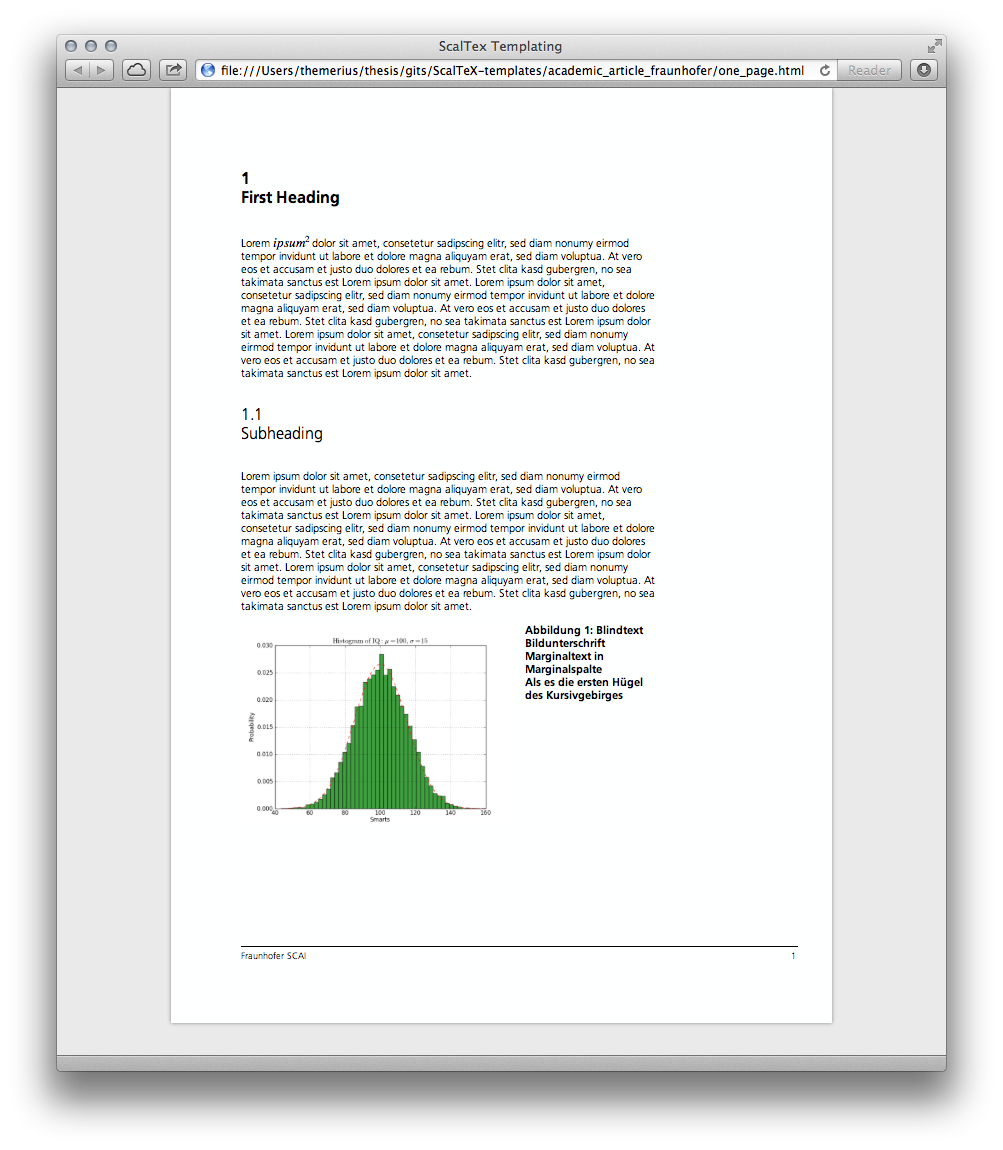
\includegraphics[width=0.9\textwidth]{figures/one_page.png}
  \caption{Einzelne DIN A4 Seite mit HTML und CSS gesetzt.}\label{fig-one_page}
\end{figure}
\newpage

\paragraph{Strategie}
Konzentriert sich zunächst darauf die Entitäten, wie Texte, Bilder usw.,
auf Seiten im Dokumentenfluss zuzuweisen. In diesem Fall darf zunächst eine
einzelne Entität nicht die größe einer Seite überschreiten -- diese
Problematik soll später näher erläutert werden.

Der prinzipielle Ablauf wird auf Abbildung \ref{fig-aufteilungsstrategie}
visualisiert. Rechts ist die temporäre \emph{Construction Page}, die zum
ausmessen der Entitäten dient, für jeden Seitentypus welcher vom jeweilige
Dokumenten-Template geboten wird gibt es also eine Construction Page, sofern
dieser sich von den Ausmaßen anderes verhalten sollte.

Der Ablauf ist also wie folgt: die Entität wird mithilfe der Construction
Page ausgemessen und wenn auf der \emph{View Page} noch genügend Platz
vorhanden ist dort hin verschoben, wenn nicht genügend Platz vorhanden ist,
wir eine neue Seite erstellt und die Entität dort platziert.

Hier kann noch ein Zwischenschritt eingefügt werden, der es ermöglichen
sollte gerade Textentitäten weiter aufteilen zu können, so dass eine
bessere Auslastung der Seiten erreicht werden kann.
% TODO Falls umgesetzt, noch ergänzen.

\newpage
\begin{figure}[h!]
  \centering
    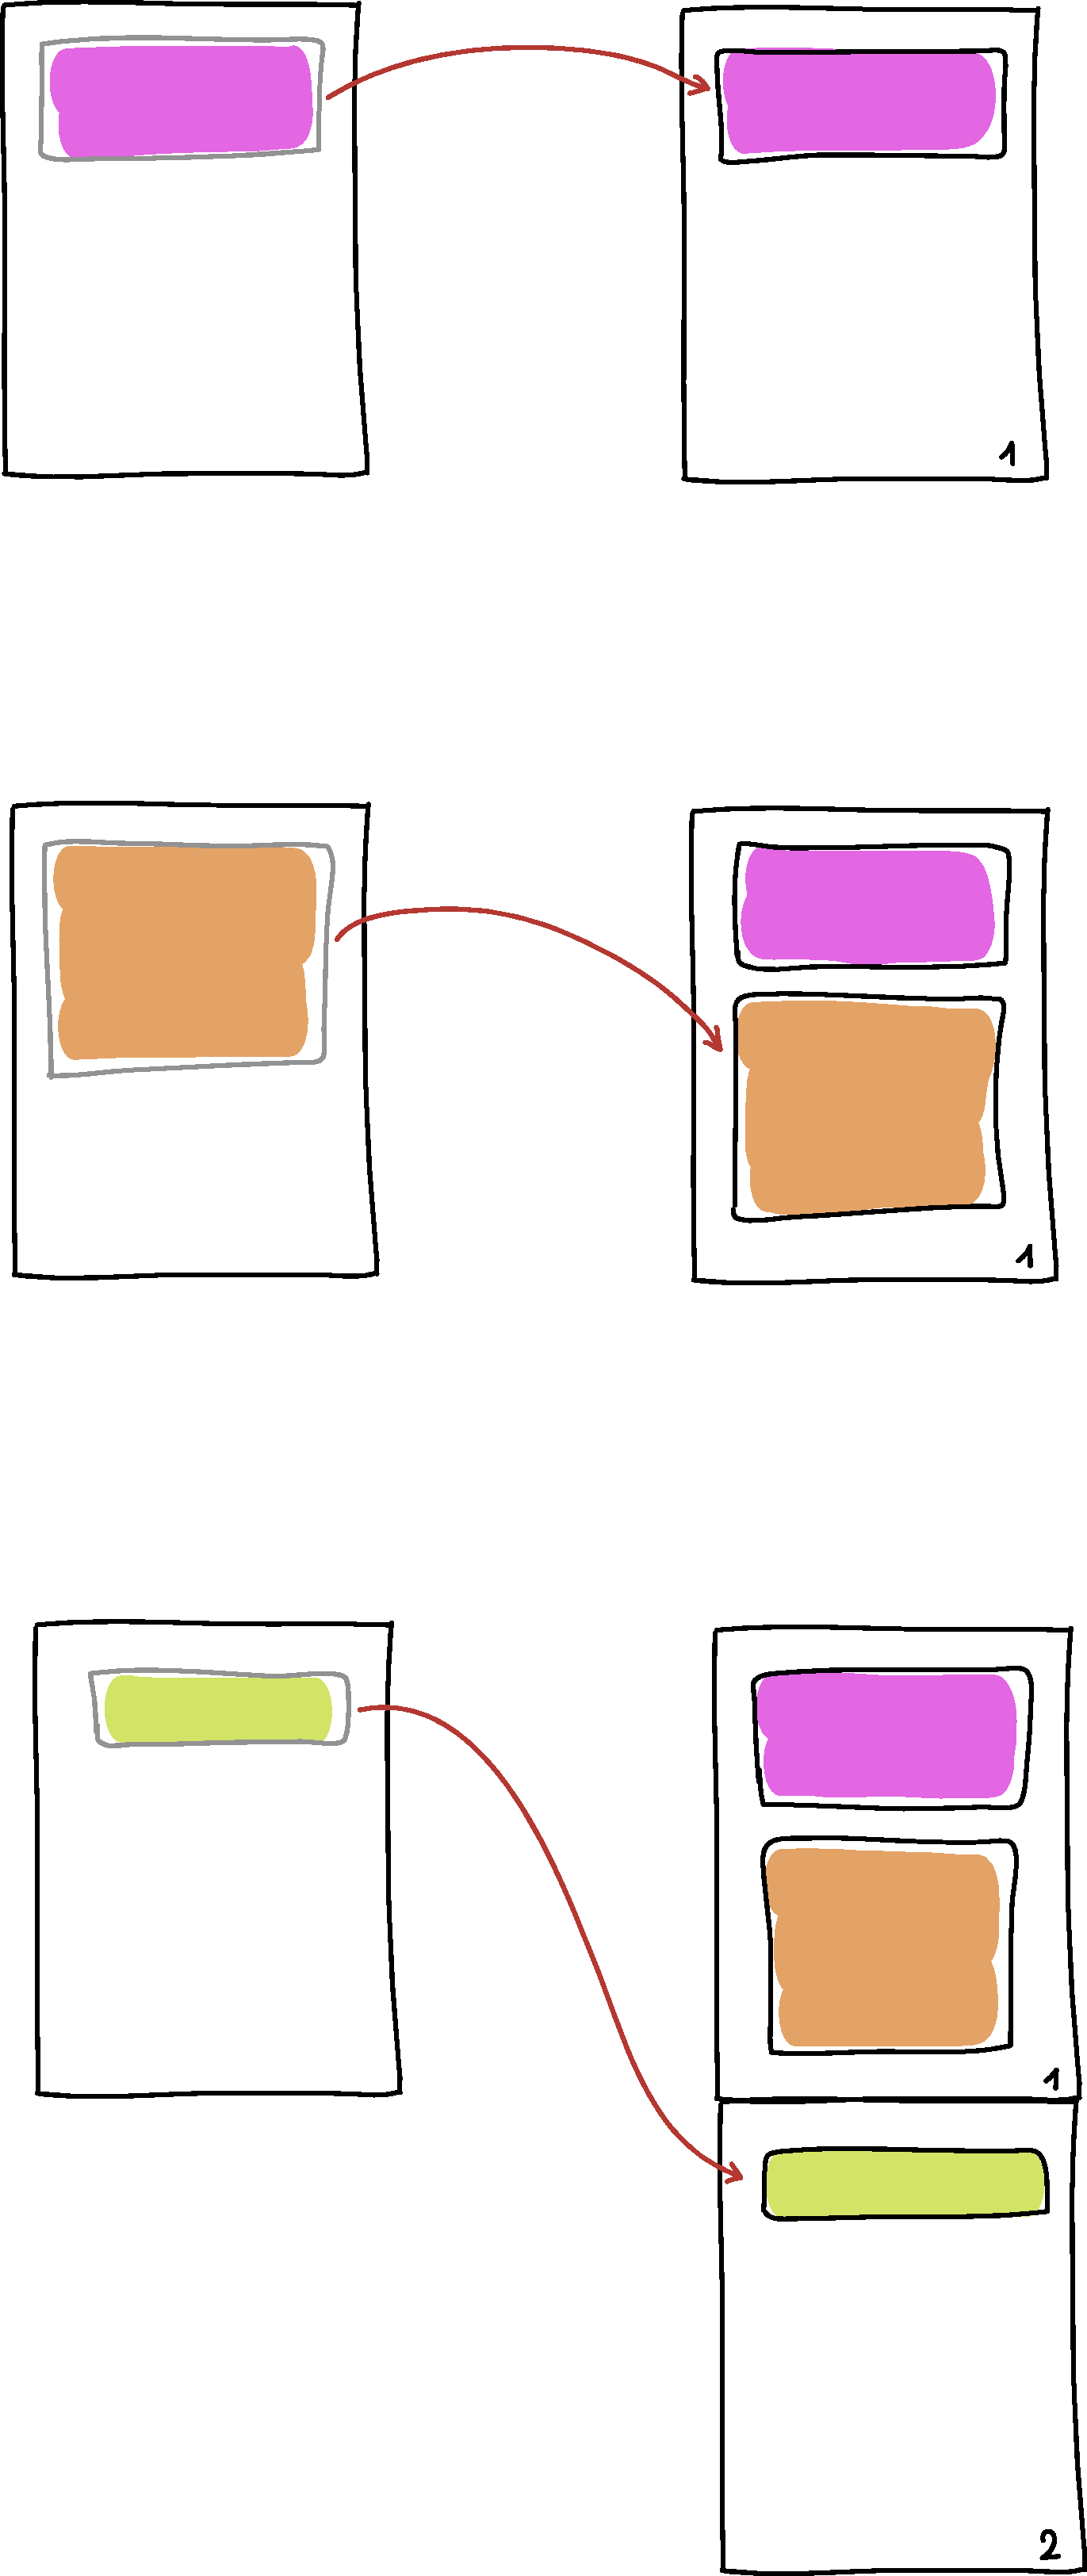
\includegraphics[height=0.9\textheight]{figures/aufteilungsstrategie.pdf}
  \caption{Aufteilungsstrategie: wie Entitäten auf einzelne Seiten
           verteilt werden.}\label{fig-aufteilungsstrategie}
\end{figure}
\newpage

\subsection{Templating}

Ich habe mich dazu entschieden das Templating vorerst mit JavaScript
vorzunehmen, also komplett auf der Seite des Dokumenten-Betrachters.
Dies soll den Zweck haben, dass ein Dokumenten-Template-Designer es
leichter haben soll sein Dokumenten-Design zu bauen und zu debuggen --
komplett unabhängig von der DSL bzw. der Programmierlogik.
Zum Einsatz kommt dabei die Javascript-Bibliothek
\emph{mustache}\footnote{\url{http://mustache.github.com}}.

Auf diese Weise kann jede einzelne Entität oder Seite clientseitig
durch ein kleines Template-Snippet darstellt werden, welches an die
Bedürfnisse des spezifischen Dokumenten-Designs bzw. Dokumenten-Templates
angepasst ist. Beispielsweise eine Überschrift, könnte so aussiehen.

\begin{verbatim}
<script id="heading" type="text/template">
<div class="row">
  <div class="col4">
    <{{h}}>{{number}}
      </br>
      {{heading}}
    </{{h}}>
    </br></br>
  </div>
  <div class="row-end">&nbsp;</div>
</div>
</script>
\end{verbatim}

Diese muss dann nur noch von der DSL entsprechend mit einer
JSON-Datenstruktur\footnote{JSON ist die \emph{JavaScript Object Notation},
und bildet die zentrale Datenstruktur von JavaScript.
Mehr Informationen unter \url{http://json.org}.} gefüttert werden.

\subsection{Dokumenten-Areale}

Die resultierenden Seiten zur Anzeige (View Pages), werden bestimmten
Arealen zugeordnet, diese dienen insbesondere der logischen Strukturierung
des Dokuments. Aus Sicht der Seiten sind diese Areale quasi
Einhängepunkte, wo die fertig befüllten Seiten angefügt werden.
Beispiele für Areale sind z.B.

\begin{itemize}
  \item Titelblätter,
  \item Inhaltsverzeichnis,
  \item eigentliches Dokument,
  \item Literaturverzeichnis,
  \item \ldots
\end{itemize}

Innerhalb des HTML-Dokuments können diese Areale in ihrer Reihenfolge
verändert werden, und ermöglichen so einen recht flexiblen Umgang mit
den Dokumtenten-Arealen. Diese sind ganz primitiver HTML-Code wie dieser
z.B.:

\begin{verbatim}
<div id="TitlepageAreal"></div>
<div id="TableOfContentsAreal"></div>
<div id="DocumentAreal"></div>
\end{verbatim}

Es muss nur dem JavaScript-Framework welches die Abstraktion für die
Seiten vornimmt mitgeteilt werden, für welche IDs, welche Areale definiert
sind.

\subsection{Klassendiagramm?}

pass  % TODO!!!

\subsection{Beispiel Code}

pass % TODO ein kleines aber komplettes html-code beispiel (welches man durch
% die vorherigen kapitel hoffentlich verstehen kann.

\section{Vorwärtsverweis „Forward Reference“}\label{sec-forwardreference}

Dieses Problem tritt auf, wenn z.B. in einem Text auf eine Abbildung
verweisen wird, welche innerhalb des Programmflusses erst später verfügbar
wird.

\begin{lstlisting}
... auf Abbildung {Reference} ist zu sehen ...

Reference = new Figure(...)
\end{lstlisting}

Hier wird also auf \lstinline|Reference| bereits zugegriffen,
bevor sie überhaupt existiert. Erschwerend kommt hinzu, dass sich die
Reihenfolge der Entitäten (Texte, Bilder, etc.) nicht verändert werden darf.
Die Abbilung soll also an der Position im Dokument erscheinen, an der sie
auch im Dokument-Quellcode geschrieben wurde, da es sich hier um eine DSL
handelt, die sich möglichst nahme am eigentlichen Dokument orientiert.

% Note:
% Von oben nach unten, wir die Lösung immer unflexibler, unsicherer und
% aufwendiger in der Implementierung. Wobei Request-Queue und Pattern-Matching
% etwas zusammengehören.


\subsection{Closure}

Insbesondere funktionale Programmiersprachen wie Scala haben die
Möglichkeit Closures zu bilden, d.h. der Teile Geltungsbereich (Scope)
der äußeren Funktion  kann von der inneren Funktion beibehalten werden,
auch wenn der Geltungsbereich der äußeren Funktion bereits verwirkt ist.
% TODO(oder in appendix?)

\begin{lstlisting}
def outer_func = {
  val v = 15
  (x: Int) => x + v  // lambda function
}
\end{lstlisting}

Auf \lstinline|v| kann noch über die Lambda-Funktion zugegriffen werden,
selbst wenn \lstinline|outer_func| nicht mehr exisiert. Teile des
\lstinline|outer_func|-Geltungsbereichts werden quasi mitgezogen.

Genau mit dieser Technik kann man den Vorwärtsverweis in den Griff bekommen.
Es wird der äußere Geltungsbereich eines Objects nach innen gezogen,
um dort später wenn alle Entitäten bekannt sind und die Referenz aufgelöst
wurde darauf zuzugreifen.

\begin{lstlisting}
object O {
  val text = () => s"… auf Abbildung $reference ist zu sehen …"
  val reference = 3
}

O.text()  // wenn reference vorhanden
\end{lstlisting}

Hier wird zudem die Eigenschaft des \lstinline|object| ausgenutzt,
dass die im \lstinline|object| genannten Variablen immer schon vom Compiler
zumindest mit einer \lstinline|null|-Referenz exisieren, aber die Reihenfolge
der eigentlichen Instanziierung wird nicht verändert. Durch das
\lstinline|lazy|-Keyword von Scala, würde die Reihenfolge modifiziert werden
und ist dadurch nicht verwendbar.

Nachteil hier ist, dass der Domänen-Benutzer innerhalb der DSL diese
\lstinline|() => s""|-Magie schreiben müsste -- was zu Verwirrung und
Unverständnis führen würde.


\subsubsection{Verbesserung für den Domänen-Benutzer}

Ideal wäre also nun eine Lösung inder der Domänen-Benutzer keine
Aufmerksamkeit auf die Closure-Magie verschwenden muss.

Wie bereits in einem vorherigen Kapitel % TODO(oder in appendix?)
erwähnt wird auf den ab Scala 2.10 verfügbaren
\lstinline|StringContext| (\lstinline|s"…"|) gesetzt.
Dieser lässt sich so erweitern, dass
sich die Closure-Magie verstecken lässt und somit in die API
gezogen wird und der Domänen-Benutzer davon gar nichts mitbekommt.

\begin{lstlisting}
implicit def byname_to_noarg[A](a: => A) = () => a

case class StringContext(parts: String*) {
  def $ (args: (() => Any)*) = () => {
    val unpacked_args = args.map(a => a())
    scala.StringContext(parts: _*).s(unpacked_args: _*)
  }
}

object O {
  val text = $"… auf Abbildung $reference ist zu sehen …"
  val reference = 3
}

O.text()  // wenn reference vorhanden
\end{lstlisting}

\lstinline|byname_to_noarg| ist eine implizite Konvertierung von einem
beliebigen Typ \lstinline|A| mit Call-by-Name
% TODO(fußzeile, appendix "benutzte scala technologien"?)
\lstinline|a: => A| in eine Lambda-Funktion \lstinline|() => a|.

\lstinline|def $| fügt die Möglichkeit hinzu \lstinline|$"…"| als individuell angepassten \lstinline|StringContext| zu verwenden. Es wird eine variable 
Argumentenliste mit den implizit zu Call-by-Name konvertierten Argumenten
aus einem beliebigen \lstinline|$"…"|-String übergeben und in ein Closure gepackt,
welches erst dann ausgeführt wird, wenn die Referenzen auch tatsächlich
vorhanden sind.

% http://stackoverflow.com/questions/13307418/scala-variable-argument-list-with-call-by-name-possible

% http://stackoverflow.com/questions/13270906/cast-scala-string-to-stringcontext-and-virtually-forward-references

\subsection{Eval}

\subsection{Datenstrukturbasierend}

\subsubsection{Request-Queue}

Nur Idee!

\subsubsection{Pattern-Matching}

Nur Idee!

\subsubsection{„place here“}

Praktikabel mit Xtext-Generator. Prototypisierung ausnutzen (C-Header).


\begin{appendix}
  \chapter{Quellcode}

Hier ist der Quellcode der im Kapitel \ref{ch-architektur} architekturell
beschrieben wurde aufgelistet.
Die Repositories worin der Code duch die git-Versionskontrolle
verwaltet werden sind auf Github gespeichert:

\begin{itemize}
  \item Zielarchitetkur: \url{https://github.com/themerius/ScalTeX-templates}
  \item DSL: \url{https://github.com/themerius/ScalTeX-DSL}
\end{itemize}

\section{Zielarchitektur}

\section{Scala DSL}


\end{appendix}

\addcontentsline{toc}{chapter}{Literaturverzeichnis}
\bibliographystyle{apalike}  % apalike
\bibliography{bib/references}

%\listoffigures
%\listoftables

\end{document}

